\section{Testing each veto against a fresh fit}
\label{sec:refit}
We asked whether a veto identifies a deletion that harms the learner when it trains again. We used 14 previously examined PMLB classification tasks and three stratified outer folds per task~\cite{romano2022pmlb}. Within each fold we sampled up to twelve distinct proposals uniformly from the union of three search paths (single-panel, nested-majority and separating-majority). Separately, we drew up to four deletion sets uniformly at each distinct admissible removal size among one, $\lceil |A|/4\rceil$ and $\lfloor |A|/2\rfloor$. All retained sets were nonempty strict subsets of the Gain-ranked anchor $A$. The 400 path and 379 drawn proposals share 75 fold--support pairs. We report the collections separately.

We recorded the proposal identities and votes, refitted XGBoost on $S$ and $A$ using all development rows, and compared the two predictions on the same outer test rows. A \emph{refit failure} occurs if the relative loss on any metric exceeds its allowance in Eq.~\eqref{eq:ballot}. The limit was 3\% for both AUC and accuracy. No fold met the rare-positive criterion for including average precision. A veto is a positive decision. The true-positive rate (TPR) is the fraction of failing refits vetoed, and the false-positive rate (FPR) is the fraction of passing refits vetoed. Both condition on an outcome measured on a finite test fold.

\subsection{Which failures do interior restorations detect?}
\begin{table}[tb]
\centering
\caption{True- and false-positive rates (\%) for a veto, with 95\% task--fold percentile intervals. Search-path proposals include 189 observed failures and 211 passes; drawn deletions include 163 and 216. Seventy-five fold--support pairs occur in both sources. Rates pool proposals within each source.}
\label{tab:operating-rates}
\small\setlength{\tabcolsep}{3pt}
\begin{tabular}{@{}lrr@{\quad}rr@{}}
\toprule
& \multicolumn{2}{c}{Search path} & \multicolumn{2}{c}{Drawn deletions} \\
Rule & TPR & FPR & TPR & FPR \\
\midrule
Empty, point & \shortstack[r]{88.4\\[-.5pt]{\scriptsize [78.6, 96.1]}} & \shortstack[r]{78.2\\[-.5pt]{\scriptsize [63.7, 88.2]}} & \shortstack[r]{92.6\\[-.5pt]{\scriptsize [85.0, 98.0]}} & \shortstack[r]{73.6\\[-.5pt]{\scriptsize [65.9, 80.5]}} \\[2pt]
Empty, four panels & \shortstack[r]{89.4\\[-.5pt]{\scriptsize [77.5, 98.7]}} & \shortstack[r]{78.2\\[-.5pt]{\scriptsize [66.4, 87.4]}} & \shortstack[r]{98.2\\[-.5pt]{\scriptsize [95.7, 100.0]}} & \shortstack[r]{75.9\\[-.5pt]{\scriptsize [68.4, 82.4]}} \\[2pt]
Both endpoints & \shortstack[r]{91.5\\[-.5pt]{\scriptsize [81.1, 99.4]}} & \shortstack[r]{82.5\\[-.5pt]{\scriptsize [72.9, 90.0]}} & \shortstack[r]{98.8\\[-.5pt]{\scriptsize [96.7, 100.0]}} & \shortstack[r]{78.2\\[-.5pt]{\scriptsize [71.1, 84.6]}} \\[2pt]
Nested minimum & \shortstack[r]{92.1\\[-.5pt]{\scriptsize [81.6, 99.4]}} & \shortstack[r]{83.9\\[-.5pt]{\scriptsize [74.7, 91.2]}} & \shortstack[r]{98.8\\[-.5pt]{\scriptsize [96.7, 100.0]}} & \shortstack[r]{79.6\\[-.5pt]{\scriptsize [72.5, 86.5]}} \\[2pt]
Separating, point & \shortstack[r]{94.7\\[-.5pt]{\scriptsize [85.3, 100.0]}} & \shortstack[r]{91.5\\[-.5pt]{\scriptsize [84.0, 96.3]}} & \shortstack[r]{98.2\\[-.5pt]{\scriptsize [95.8, 100.0]}} & \shortstack[r]{81.0\\[-.5pt]{\scriptsize [74.5, 87.8]}} \\[2pt]
Separating, pooled & \shortstack[r]{82.5\\[-.5pt]{\scriptsize [67.2, 94.3]}} & \shortstack[r]{65.9\\[-.5pt]{\scriptsize [50.6, 79.1]}} & \shortstack[r]{93.9\\[-.5pt]{\scriptsize [85.4, 98.6]}} & \shortstack[r]{68.5\\[-.5pt]{\scriptsize [58.5, 77.5]}} \\[2pt]
Separating minimum & \shortstack[r]{97.4\\[-.5pt]{\scriptsize [92.4, 100.0]}} & \shortstack[r]{91.9\\[-.5pt]{\scriptsize [85.6, 96.2]}} & \shortstack[r]{98.8\\[-.5pt]{\scriptsize [96.7, 100.0]}} & \shortstack[r]{82.4\\[-.5pt]{\scriptsize [76.1, 88.7]}} \\[2pt]
Random minimum & \shortstack[r]{96.3\\[-.5pt]{\scriptsize [89.5, 100.0]}} & \shortstack[r]{92.9\\[-.5pt]{\scriptsize [85.2, 97.6]}} & \shortstack[r]{98.8\\[-.5pt]{\scriptsize [96.7, 100.0]}} & \shortstack[r]{84.7\\[-.5pt]{\scriptsize [79.3, 90.1]}} \\[2pt]
\bottomrule
\end{tabular}
\end{table}


On the search paths, 189 of 400 refits failed. Requiring a majority at every separating restoration vetoed 184 of these failures and 194 of the 211 passes (Table~\ref{tab:operating-rates}). Relative to the two endpoint restorations, the interiors caught 11 additional failures and rejected 20 additional passes. The paired changes in TPR and FPR were $+5.82$ percentage points (95\% interval $[0,13.56]$) and $+9.48$ points ($[4.57,15.14]$). On drawn deletions, 163 of 379 refits failed. The interiors caught zero additional failures and vetoed nine additional passes. The corresponding changes were 0 points ($[0,0]$) and $+4.17$ points ($[0.46,9.14]$). The zero-width interval reflects agreement on every failing refit available to resample. Appendix Table~\ref{tab:refits} gives the original confusion counts.

We pooled counts before computing the rates. For the pointwise 95\% intervals, each of 30,000 bootstrap draws sampled 14 tasks with replacement and three folds with replacement per sampled task. Each fold carried all its proposals, outcomes and decisions together. Every rule used the same draws, and each difference was computed within draw. Outer training sets overlap~\cite{bengio2004variance}. Resampling whole tasks with their folds intact gave path intervals of $[0.72,12.16]$ points for the increase in TPR and $[5.56,12.89]$ for the increase in FPR. These intervals describe reweighting the observed tasks and folds with their models, votes and test outcomes fixed. Giving each task and fold equal mass before conditioning on failure changed the path increases to 3.85 and 9.26 points.

\begin{figure}[tb]
\centering
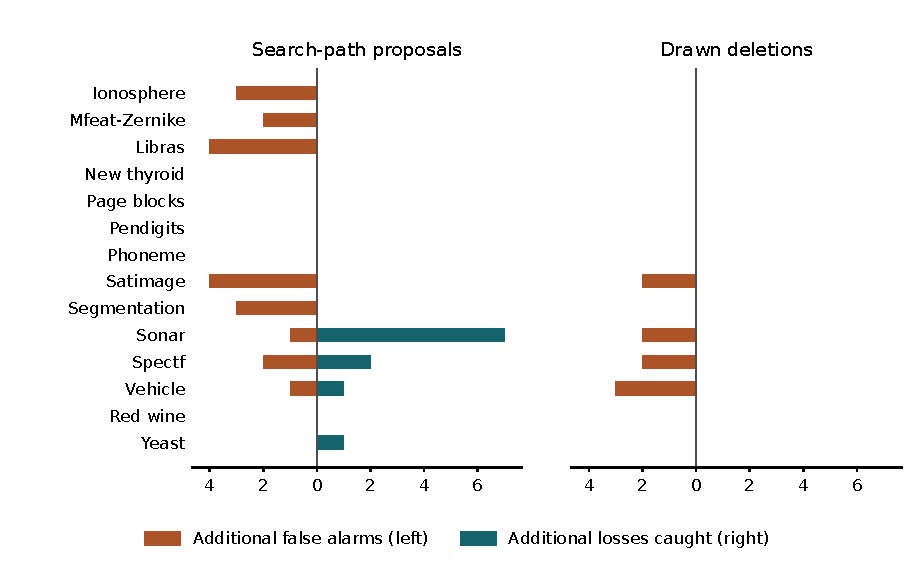
\includegraphics[width=\linewidth]{figures/refit-vetoes.pdf}
\caption{Additional XGBoost vetoes from testing separating interiors after both endpoints passed. Bars count outer refits within tolerance (left) or exceeding tolerance (right).}
\label{fig:vetoes}
\end{figure}

\paragraph{Changing the voting rule or learner.}
On the same 704 distinct fold--support pairs we crossed five restoration families, two aggregation rules, three panel counts, four approval quorums and three vote-side loss allowances. The 360 settings per voting learner include equivalent rules. A pooled rule takes the approval fraction over all panel--restoration pairs. A minimum rule requires the specified fraction within every restoration. The first of 1, 4 or 12 panels used the original ranking rows and the others reweighted those rows. The outer failure criterion stayed fixed at 3\% throughout.

\begin{table}[tb]
\centering
\caption{True/false veto counts after changing one aspect of the four-panel separating minimum. Each learner judges its own refits. The proposal-side tolerance varies only in the last two rows. The outer tolerance stays fixed. Logistic refits exceeded it in 216 of 400 path and 187 of 379 drawn proposals.}
\label{tab:operating-rules}
\small\setlength{\tabcolsep}{3pt}
\begin{tabular}{@{}lrr@{\quad}rr@{}}
\toprule
&\multicolumn{2}{c}{XGBoost}&\multicolumn{2}{c}{Logistic regression}\\
Rule & Path & Drawn & Path & Drawn \\
\midrule
Both endpoints & 173/174 & 161/169 & 211/159 & 182/144 \\
Separating minimum & 184/194 & 161/178 & 213/176 & 184/173 \\
Pooled votes & 156/139 & 153/148 & 203/122 & 174/124 \\
One panel & 179/193 & 160/175 & 212/172 & 183/169 \\
Twelve panels & 184/191 & 161/177 & 213/178 & 183/171 \\
Ties accepted & 178/186 & 161/171 & 212/168 & 183/162 \\
Vote tolerance 1\% & 184/204 & 162/201 & 216/182 & 187/189 \\
Vote tolerance 5\% & 174/166 & 157/162 & 211/159 & 180/155 \\
\bottomrule
\end{tabular}
\end{table}


Pooling XGBoost votes on paths reduced false alarms from 194 to 139 and detections from 184 to 156 (Table~\ref{tab:operating-rules}). At vote-side tolerances of 1\%, 3\% and 5\%, adding separating interiors to endpoints gave 3/11, 11/20 and 21/21 additional detections/false alarms on paths. On drawn deletions the additions were 1/8, 0/9 and 6/11. At 3\%, twelve panels gave the same total detections as four in both collections and fewer false alarms (191 versus 194 on paths and 177 versus 178 on drawn deletions). Thus twelve panels had lower observed error cost at every finite miss cost if computation is free.

Changing the refitted learner to standardized L2 logistic regression ($C=1$) changed the failure label on 111/400 path and 82/379 drawn proposals. With XGBoost votes held fixed, switching from XGBoost to logistic refits changed the additional detections/false alarms from 11/20 to 8/23 on paths and from 0/9 to 1/8 on drawn deletions. With logistic votes held fixed, the same switch changed 7/12 to 2/17 and 4/27 to 2/29. Each comparison used the same tree-derived proposals, restorations, four panels, majority and 3\% tolerance.

\subsection{When is an additional veto worth its cost?}
Let a veto of a passing refit cost one unit and a missed refit failure cost $r$. With $N$ proposals the observed mean cost is $(\mathrm{FP}+r\,\mathrm{FN})/N$. On paths, separating incurs lower cost than endpoints exactly when $r>20/11=1.82$ (rounded). Sonar contributed seven of the eleven extra detections (Fig.~\ref{fig:vetoes}). Omitting Sonar raises the crossover to $19/4=4.75$. The paired task/fold bootstrap gave a crossover range of $[0.46,\infty]$, accounting for resamples with extra false alarms and zero extra detections. Keeping each task's folds intact gave $[0.56,19.00]$. On drawn proposals the additional nine false alarms favor endpoints at every finite $r$.

Against the other seven original masking rules and both constant decisions, the four-panel separating minimum had lowest pooled path cost for $1.96\lesssim r\le3.40$. Including a simple size rule changes that conclusion. Separating beats never vetoing for $r>194/184$, vetoing everything for $r<17/5$, and vetoing deletion of at least one quarter of the anchor for $r>68/19$. Thus the quarter-deletion rule or veto-all is cheaper at every $r$ on the pooled paths. The corresponding inequalities on drawn proposals are $r>178/161$, $r<19$ and $r>62/18$, and endpoints still dominate separating. With equal mass per task and fold, separating has lowest path cost for $3.28\lesssim r\lesssim3.93$ within this library of eight original rules, two constants and one size rule.

If the failure prevalence changes to $p$ while conditional rates transfer, the expected cost is $(1-p)\mathrm{FPR}+r p(1-\mathrm{TPR})$~\cite{provost2001robust}. For the path rates, lowering $p$ from the observed 47.25\% to 25\% raises the separating-versus-endpoint crossover to 4.89. At 10\% it reaches 14.66. These error costs price a decision on one proposal. The cost of computing masks and the consequences for later search steps require separate accounting.

\paragraph{Choosing a rule on other tasks.}
We next chose the lowest-cost rule on thirteen tasks and applied it to the omitted fourteenth, repeating the procedure separately for each cohort and each $r\in\{1,2,5,10\}$. The two libraries contained all 360 masking rules or six deletion-fraction cutoffs ($1/12,1/6,1/4,1/3,1/2,3/4$), each with both constant decisions. Ties favored constants, then cheaper masking rules or larger size cutoffs. At equal costs the selected mask and size policies made 159 and 170 errors on paths, against 183 and 98 on drawn deletions. The one-third cutoff was selected in every training set for drawn deletions and beat the selected mask rule on 12 of 14 held-out tasks. Removing each task from both training and evaluation and repeating the procedure reversed the sign of the path comparison for some omissions at every $r$. The size library kept its lower drawn cost under every omission at $r=1,2,5$. These are retrospective comparisons on the previously inspected task collection.
